\documentclass[tikz,border=10pt]{standalone}
\usepackage{tikz}
\usepackage{verbatim}
\begin{document}
	\usetikzlibrary{arrows,positioning} 
	\tikzset{
		%Define standard arrow tip
		>=stealth',
		% Define arrow style
		pil/.style={
			->,
			thick,
			shorten <=2pt,
			shorten >=2pt,}
	}
	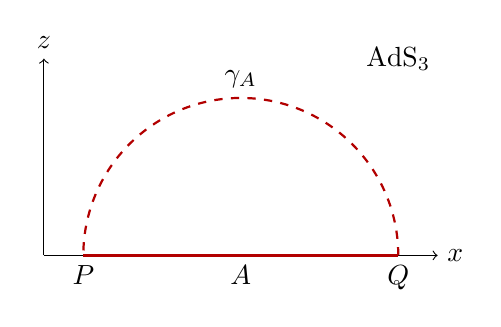
\begin{tikzpicture}
	\draw[->] (0,0)--(5,0)node[anchor=west]{$x$};
	\draw[->] (0,0)--(0,2.5)node[anchor=south]{$z$};
	\draw[red!70!black, dashed,thick] (4.5,0) arc [start angle =0, end angle = 180, radius =2];
	\draw[red!70!black,thick]  (0.5,0)--(4.5,0);
	\draw (2.5,0) node[anchor = north]{$A$};
	\draw (0.5,0) node[anchor = north]{$P$};
	\draw (4.5,0) node[anchor = north]{$Q$};
	\draw (2.5,2) node[anchor = south]{$\gamma_A$};
	\draw (4.5,2.5) node{AdS${}_3$};
	\end{tikzpicture}
\end{document}